\documentclass[11pt]{article}
\usepackage{fullpage}

\usepackage{amsmath}
\usepackage{graphicx} \usepackage{natbib}
%\usepackage{colortbl}
\usepackage{subfigure} \usepackage{epsfig}

\usepackage{pdfpages}
\usepackage{url}
\usepackage{color}   %May be necessary if you want to color links
\usepackage{hyperref}
\hypersetup{
    colorlinks=true, %set true if you want colored links
    linktoc=all,     %set to all if you want both sections and subsections linked
    linkcolor=blue,  %choose some color if you want links to stand out
}

\usepackage{listings}
\usepackage{color}

\definecolor{dkgreen}{rgb}{0,0.6,0}
\definecolor{gray}{rgb}{0.5,0.5,0.5}
\definecolor{mauve}{rgb}{0.58,0,0.82}

\lstset{frame=tb,
  language=Java,
  aboveskip=3mm,
  belowskip=3mm,
  showstringspaces=false,
  columns=flexible,
  basicstyle={\small\ttfamily},
  numbers=none,
  numberstyle=\tiny\color{gray},
  keywordstyle=\color{blue},
  commentstyle=\color{dkgreen},
  stringstyle=\color{mauve},
  breaklines=true,
  breakatwhitespace=true
  tabsize=3
}
\makeatletter
\newcommand\footnoteref[1]{\protected@xdef\@thefnmark{\ref{#1}}\@footnotemark}
\makeatother

\title{CMC Startup Instructions}
%\author{
%   Meagan Morscher
%}
%\date{\today}

\begin{document}
\maketitle


\tableofcontents
\newpage

%=============================================================================================================


\section{Introduction to the Code}
This is code offers one approach for solving the gravitational {\it N}-body problem. The basic problem is as follows: you have a system of {\it N} particles (stars, in our case) and they are all interacting with one another via the gravitational force. How does the system evolve over time? There are several ways to solve the {\it N}-body problem, each method having its pros and cons. The two most common methods in use today are the directy {\it N}-body method and the Monte Carlo method. Our code uses the MC method. We will discuss them both briefly before moving into a more detailed discussion of our MC technique.

In the direct {\it N}-body method, the equations of motion for each star are solved via numerical integration. Each star feels a gravitational pull from all N-1 other stars, and in each timestep, its position and velocity is updated according to the net force it feels over that timestep. This is the most exact method of solving the N-body problem, but it has its costs: the computation time scales as {\it N\,}$^2$. The MC method is a simplified way to solve the N-body problem that makes use of three assumptions that are appropriate for the case of globular clusters: physics dominated by two-body relaxation, spherical symmetry

Monte Carlo (MC) methods calculate the dynamical evolution of a collisional system of N stars in the Fokker-Planck approximation, which applies when the evolution of the cluster is dominated by two-body relaxation, and the relaxation time is much larger than the dynamical time. In practice, further assumptions of spherical symmetry and dynamical equilibrium have to be made. The Henon MC technique (Henon 1971), which is based on orbit averaging, represents a balanced compromise between realism and speed. The MC method allows for a star-by-star realization of the cluster, with its N particles representing the N stars in the cluster. Integration is done on the relaxation timescale, and the total computational cost scales as O(NlogN) (Henon 1971).

Our code here is based on the Henon-type MC cluster evolution code CMC (Cluster Monte Carlo), developed over many years by Joshi et al. (2000, 2001), Fregeau et al. (2003), Fregeau \& Rasio (2007), Chatterjee et al. (2010), and Umbreit et al. (2012). CMC includes a detailed treatment of strong binary star interactions and physical stellar collisions (Fregeau \& Rasio 2007), as well as an implementation of single and binary star evolution (Chatterjee et al. 2010) and the capability of handling the dynamics around a central massive black hole (Umbreit et al. 2012).

%=============================================================================================================

\section{Code Description}
The principal data structure is an array of structures of type star\_t. One or more of these stars can be binaries. Binaries are stored in a separate array of structures of type binary\_t. If an element in the star array is a binary, it's binind property/variable is assigned a non-zero value. Moreover, the value of this variable is assigned in such a way that it indicates the index of the binary array which holds the properties of this binary. A detailed description of our code can be found in our aforementioned papers, here we present a flowchart and pseudocode which will assist in understanding it.

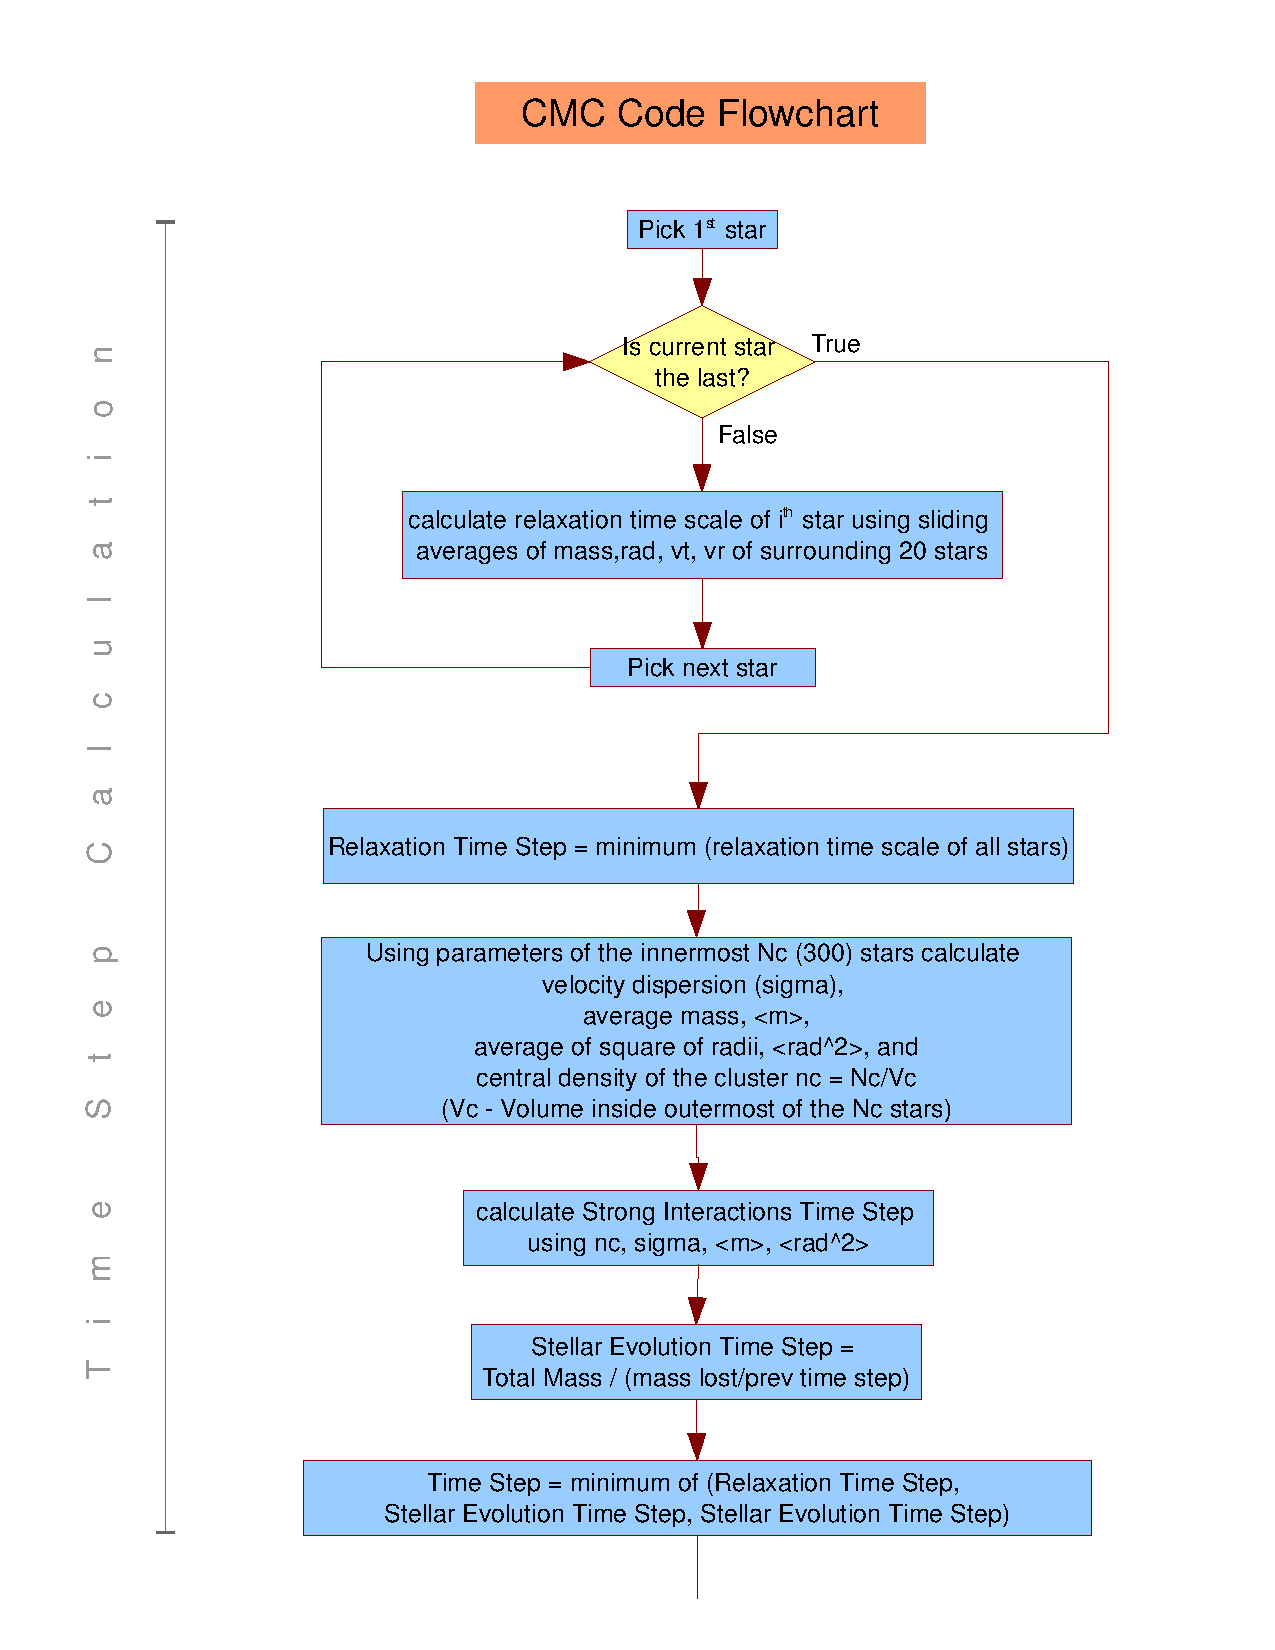
\includepdf[pages=-]{Flowchart_CMC.pdf}
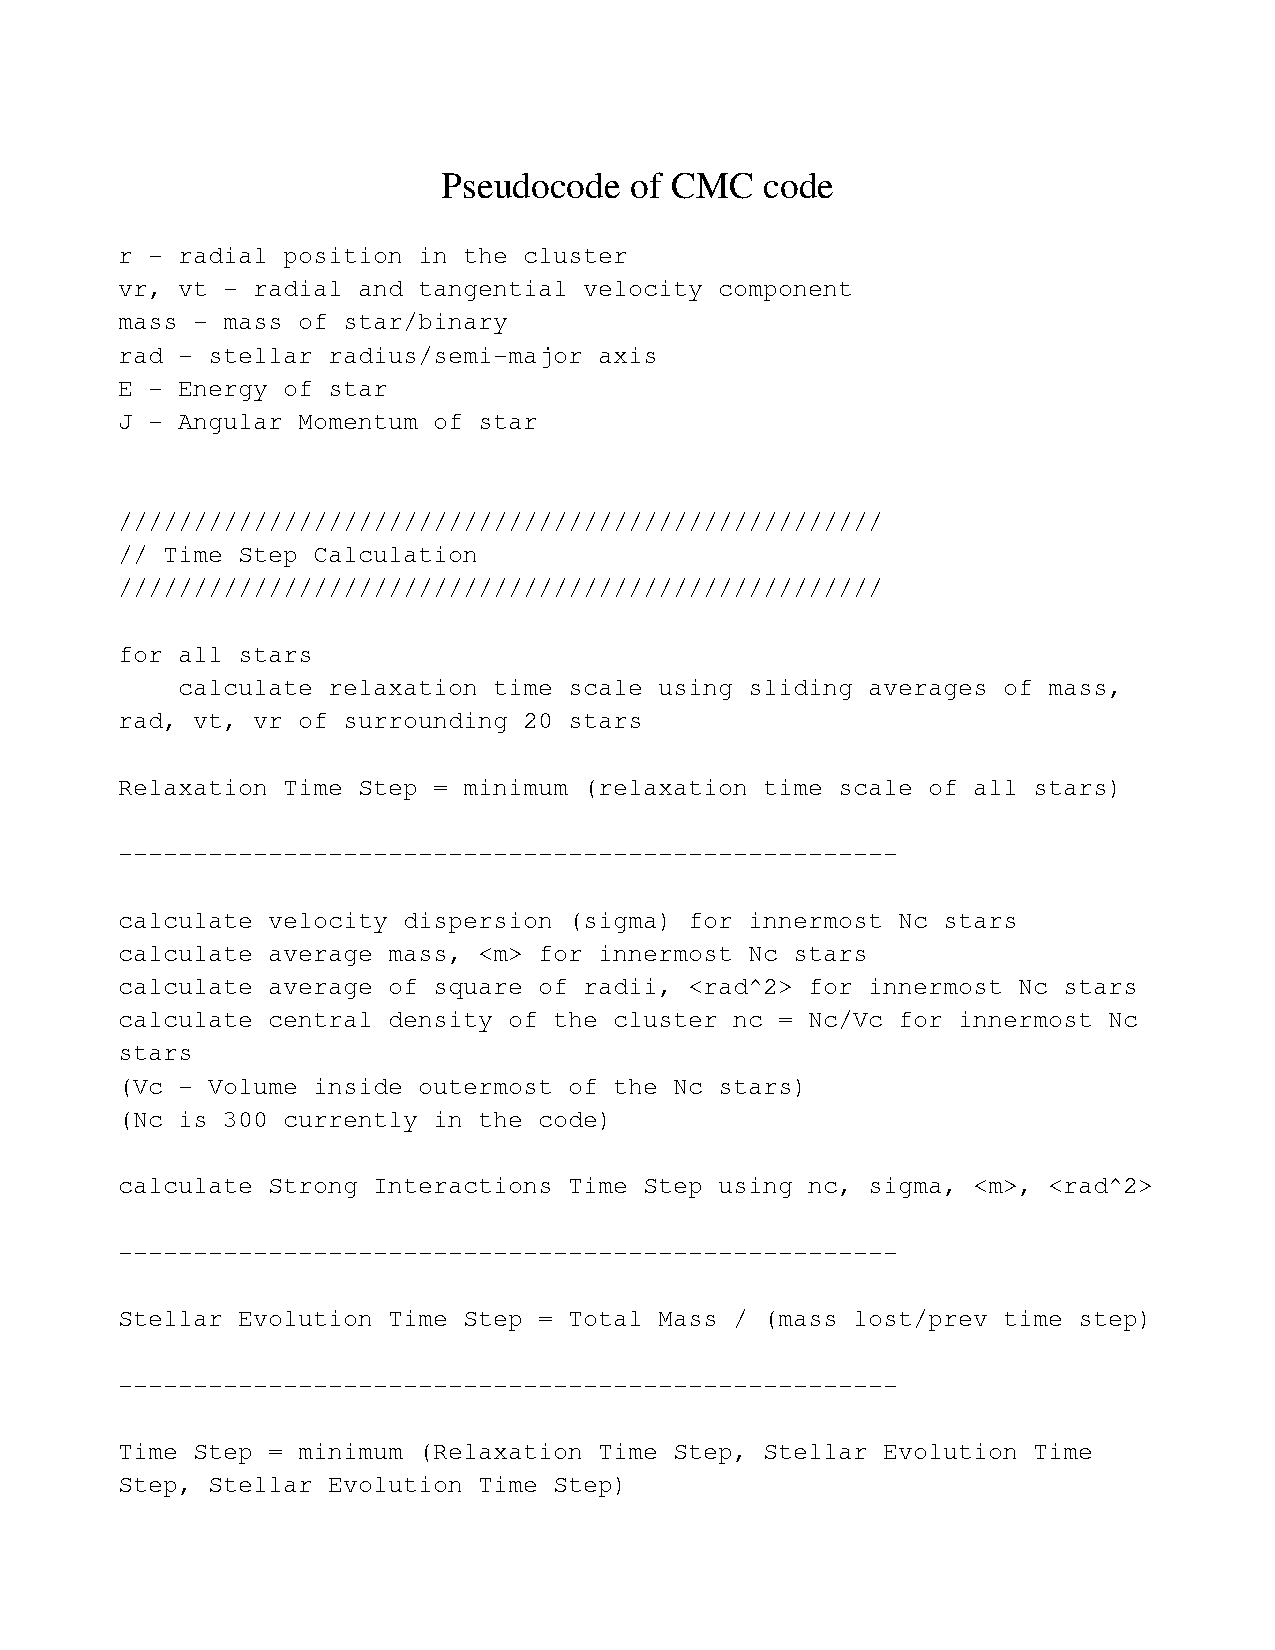
\includepdf[pages=-]{Pseudocode_CMC.pdf}

Following is a discussion about the parallelization details of the code, primarily to assist developers.

\subsection{Parallelization Strategy}
There are various routines which have varying dependencies and accesses between elements of the data structures. To minmize inter-process communication required by these routines as much as possible, we partition the data such that the number of stars held by each processor is a multiple of MIN\_CHUNK\_SIZE (input parameter, defaults to 20, refer to our paper\footnote{\label{note_paper}\url{http://adsabs.harvard.edu/abs/2013ApJS..204...15P}} for a justification for the choice of this value, and detailed explanation). The remainder of stars (which is $<$ MIN\_CHUNK\_SIZE) after division goes to the last processor.

Most routines do computations on a star by star basis, and access only the properties of the star being processed. However, the values of gravitational potential, masses of the stars and radial positions of the stars are accessed in a complex, data-dependent manner throughout the code. Hence, we store these values in separate arrays and duplicate/copy these across all processors. Since these properties change during a timestep, we synchronize these arrays at the end of each time step.

Like mentioned above, most routines perform computations on a star by star basis. The only routine that differs from this pattern is the sorting routine that sorts all the stars by their radial positions. We use a parallel sorting algorithm called Sample Sort (see our paper\footnotemark[\value{footnote}] for a detailed discussion).

The parallel sorting routine does the sorting and automatically redistributes the data to the processors, however, there is no control over the number of stars that will end up on each processor. So, after the sorting takes place, we exchange data between processors to adhere to the data partitioning scheme mentioned above.

\subsection{Programming Guidelines for Developers}
It is very necessary to read our paper\footnotemark[\value{footnote}] before proceeding. The paper covers most of the code and parallelization aspects which in itself serves as a guide for development. Here, we cover some more low level coding details to aid a developer who wants to modify the code. An introduction to MPI might also be very useful, and in fact necessary for any non-trivial code development. 

The parallelization follows a SIMD model. Any line of code is executed by all processors. Unlike a sequential code, variables might have different values on different processors. A simple example is the variable $myid$ which stores the ID of the processor. If p processors are used, the IDs go from $0$ to $p-1$, and each processor will contain the value of its ID in this variable. On the other hand the variable $procs$ stores the total number of processors used. One can see that the variable $procs$ will have the same value on all processors whereas $myid$ will have different value depending on the processor.

The data/stars are initially partitioned, after reading from the input file, into the user specified number of processors. The partitioning scheme is described in detail in the paper, and is chosen in such a way as to minimize communication required during the program execution. Binaries are partitioned among processors as well, and are indexed similar to the serial code i.e. the variable $binind$ of a star, if greater than 0, refers to the index of the corresponding binary in the binary array.

The variables $mpiBegin$, $mpiEnd$, and the arrays $Start$ and $End$ are used to implement and store the data partitioning scheme. These are used in almost every routine of the code. Let us try to understand these with an example. Say, we start with an initial of 10000 stars, and 4 processors. The data is partitioned, and each processor has 2500 stars. These are stored in the star array. Please note that in each timestep all the stars are sorted by their radial position. So, positions of all stars in processor 0 are lesser than those in processor 1 which in turn are lesser than the ones in processor 2 and so on. Now, each local array is indexed from 1 to 2500. However, if you imagine an array containing the entire set of 10000 stars, the indices of the stars local to a processor will have a different index, which will depend on the processor ID, in this imaginary global array. For instance the local stars 1 to 2500 in processor 1 will have a ``global" index 2501 to 5001. This ``global" index is require at various points in the code since some routines need some quantities of the entire set of stars. These quantities (mass, positions and potential) are duplicated across all processors, please see paper\footnotemark[\value{footnote}] for a detailed description. The variables $mpiBegin$ and $mpiEnd$ store the global index of the first and the last star in a given processor. For our example, in processor 0, these will be 1 and 2500 (the 0th star is always left out as it is marked as a sentinel); for processor 1 these will be 2501 and 5001 and so on. The $Start$ and $End$ arrays store these values of all the processors. $Start[myid]$ essentially is the same as $mpiBegin$, and $End[myid]$ has the same value as $mpiEnd$. In addition there are the $mpiDisp$ and $mpiLen$ arrays which also store essentially the same information but as displacement offsets and lengths, but these are used only at very few places.

The total number of stars in a given processor can be obtained by $mpiEnd-mpiBegin+1$. $clus.N\_MAX$ represents the current total number of stars in the simulation, whereas $clus.N\_MAX\_NEW$ is the total number of local stars in the processor i.e. $mpiEnd-mpiBegin+1$. The function $mpiFindIndicesCustom()$ sets $mpiBegin$ and $mpiEnd$, whereas $findLimits()$ populates the $Start$ and $End$ arrays. When one iterates over the local number of stars, and given a star $i$, one can get its global index using the function $get\_global\_idx(i)$.

The random number generation is parallelized, and all details are hidden, so a developer does not have to mess with the details as long as one follows a similar rng calls as an already existing one.

While introducing any new code, think in parallel. For instance say you are calculating some cumulative quantity like:

\begin{lstlisting}
   for(i=1; i<=clus.N_MAX_NEW; i++) {
      Q = star[i].a + star[i].b;
   }
\end{lstlisting}

This might appear as if it's correct, although when this runs in parallel it is far from it. $Q$ will only contain the local sum $Q$ for each processor. After this one needs to aggregate $Q$ across all processors. For this you'll have to use either $MPI\_Reduce$ or $MPI\_Allreduce$ depending on whether you want the aggregated quantity Q on one or all of the processors. This is probably the simplest use of parallel programming and use of MPI. For more complex operations which involve complex data dependencies such as communicating neighbors/ghost particles, gathering, scattering data etc., one might need to have more expertise in parallel programming using MPI. So, a tutorial on MPI is strongly advised before adding any non-trivial piece of code.

I/O:
Output is another part which one might need to add, and is non-trivial to do in parallel. However, we have introduced a decently good framework to do parallel output so the programmer doesn't have to delve into the MPI IO details. If a file needs to be written by only one node, it's simple. Just do:

\begin{lstlisting}
   if(myid == <NODE_ID>)
   {
      FILE *fp;
      fopen(...);
      fprintf(...);
      fclose(...);
   }
\end{lstlisting}

Sometimes, the data that needs to be written out might be distributed across nodes. Provided these are ASCII data files with file sizes of a few KBs to MBs (such as log files, and not snapshots which write out nearly entire data) one can use MPI IO to write them out in parallel. An example is as follows:

\begin{lstlisting}
   MPI_File mpi_binfp;
   char mpi_binfp_buf[10000], mpi_binfp_wrbuf[10000000];
   long long mpi_binfp_len=0, mpi_binfp_ofst_total=0;
   sprintf(filename, "a_e2.%04ld.dat", tcount);
   MPI_File_open(MPI_COMM_MC, filename, MPI_MODE_CREATE | MPI_MODE_WRONLY, MPI_INFO_NULL, &mpi_binfp);
   MPI_File_set_size(mpi_binfp, 0);

   for (j=1; j<=clus.N_MAX; j++) {
      if (star_array[j].binind) {
         parafprintf(binfp, "%g %g\n", binary_array[star_array[j].binind].a, sqr(binary_array[star_array[j].binind].e));
      }
   }
   mpi_para_file_write(mpi_binfp_wrbuf, &mpi_binfp_len, &mpi_binfp_ofst_total, &mpi_binfp);
   MPI_File_close(&mpi_binfp);
\end{lstlisting}

The files are opened by all processors using MPI-IO. Each processor writes the data into a string/char buffer. At the end of the timestep, all processors flush the data from the buffers into the corresponding files in parallel using MPI-IO. The code uses 5 variables for this process - the MPI-IO file pointer, which follows the format $mpi\_<fptr\_name>$, 2 char buffers, which have the format $mpi\_<fptr\_name>\_buf$ and $mpi\_<fptr\_name>\_wrbuf$, and an int/longlong variables to maintain the length of the buffer (format $mpi\_<fptr\_name>\_len$) and the offset in the file (format $mpi\_<fptr\_name>\_ofst\_total$) where data has to be written. Given all these variables, a call to the function $parafprintf(<fptr\_name>, <args>)$ which follows a pattern similar to $fprintf$, but underneath writes the given args to the respective buffers and updates the offsets etc. Once all writing has been done, each processor has different data in their respective buffers which needs to be flushed out into the file. A call to $mpi\_para\_file\_write()$ takes care of this.


\section{Before installing CMC}

Here are some things you will need to have installed on your machine in order to use CMC. If you will be running CMC on a high-performance computing cluster, many of the items below may already be installed. You will likely still have to install CFITSIO, as this is an astronomy-specific library.
\begin{enumerate} 

\item \textbf{Installation on your personal computer or laptop}

\begin{itemize}

\item \textbf{Subversion (SVN)} - \url{subversion.apache.org}

This is a version-control software that will allow you to easily download CMC, as well as install updates to CMC later on.

\item \textbf{CFITSIO library} - \url{http://heasarc.gsfc.nasa.gov/fitsio/})

This library has routines that allow you to read and write  FITS files, a commonly used data format in astronomy. CMC uses the FITS file format for providing initial conditions for a simulation.

\item \textbf{GNU Scientific Library (GSL)} - \url{http://www.gnu.org/software/gsl/}


Numerical library for C/C\verb!++! 
\item \textbf{Autoconf} - \url{http://www.gnu.org/software/autoconf/}
autoconf, automake, libtool
Automatically configures software source code packages for your operating system. CMC requires version 2.59 or later. 

\end{itemize}

\item \textbf{Installation on a high-performance computing (HPC) cluster}

If you will be running CMC on Northwestern's high-performance computing cluster, Quest, you need only install CFITSIO, as the other required software/libraries are already installed. Download CFITSIO from the website (given above) and copy the .tar file to your home directory on Quest. Cfitsio installs in its own directory by default and all you have to do to ensure that CMC can find it is to set the following environment variable in your .bashrc file:

{\addtolength{\leftskip}{10mm} 
\texttt {export PKG\_CONFIG\_PATH=\$PKG\_CONFIG\_PATH:$<$path to cfitsio directory$>$}

}
%\$PKG_CONFIG_PATH:$<$path to cfitsio directory$>$
%export PKG_CONFIG_PATH=$PKG_CONFIG_PATH:$HOME/local/cfitsio

\end{enumerate}
%\end{itemize}

%=============================================================================================================


\section{Checking out a copy of CMC}
Before checking out a copy of CMC, you will need to have to gain permission to access CMC from our web server. Contact George Campbell (daishi@northwestern.edu) set this up. After this is done, you can checkout a copy of CMC.

\begin{itemize}
\item \textbf{Checking out a copy CMC}

You will need to use your net-id to access the CMC repository. From the directory you would like to install CMC, execute the following at the command line:

{\addtolength{\leftskip}{10mm} 
\texttt{svn checkout svn+ssh://$<$your netid$>$@svn.wcas.northwestern.edu/var/svn/cmc}

}

You will be prompted to enter your password (sometimes more than once), and then the download should start. If the checkout is successful, you should see a message stating that you have ``Checked out revision XXX." 

If you type `ls' you should now see a directory called `cmc'. Type `cd cmc/branches' to move into the main CMC directory. CMC has many different \emph{branches} or versions of the code. Type `ls' to see them all. The two that may be of most interest are `cmc-springcleaning,' which is our most up-to-date serial version of the CMC code, and `cmc-mpi,' which is the parallel version of CMC, still a work in progress. The parallel version can be used for very simple models, such as running a simple plummer sphere to core collapse. Depending on which version you wish to use, the setup procedure will be slightly different.


\item \textbf{Configure and Compile}

You are now ready to configure and compile CMC. Quest has a way of allowing


In order to run jobs on the MRI nodes (i.e. the special sub-cluster belonging to the astrophysics group) on Quest, you must log onto and submit the job from a particular node (node 6). You will also have to compile CMC on the same node to ensure that everything is configured properly to run on the MRI nodes. To log onto quser06 type

{\addtolength{\leftskip}{10mm} 
\texttt{ssh -CXY quser06}

}
The shell prompt should show

{\addtolength{\leftskip}{10mm} 
\texttt{[$<$net-id$>$@quser06 $\sim$]\$}

}
You will have to navigate back to the cmc-springcleaning directory (when you ssh into quser06, it places you back in your home directory). 
Now that you are within the cmc-springcleaning branch, you will find README and INSTALL files which provide useful information about configuring and installing CMC. Below is the most basic installation procedure. From the command line, enter the following four commands:

{\addtolength{\leftskip}{10mm} \texttt{autoreconf -ivf}

\texttt{./configure}

\texttt{make}

\texttt{make install}

}
%\texttt{[$<$net-id$>$@quser06 cmc-mpi]\$} autoreconf -ivf
%
%\texttt{[$<$net-id$>$@quser06 cmc-mpi]\$} ./configure
%
%\texttt{[$<$net-id$>$@quser06 cmc-mpi]\$} make
%
%\texttt{[$<$net-id$>$@quser06 cmc-mpi]\$} make install

If there are no errors along the way, you should have an executable file called `cmc' within your current directory.

\end{itemize}

%=============================================================================================================


\section{Running CMC}
To be completed soon...
\begin{itemize}
\item Generating input files
\item Starting a simulation
\end{itemize}




\end{document}
